\section{Adatbázisok}
Adatbázisnak nevezzük azokat a nagy mennyiségű adatokat amelyek közös jellemzőkkel és struktúrákkal rendelkeznek. Az adatbázisokon belül több fajta műveletet tudunk elvégezni: karbantartás, tárolás, lekérdezés, szerkesztés, módosítás és nem utolsó sorban az adatok törlése is egy lehetőség. Ezen funkciókat egy adatbázis kezelő rendszer segítségével tudjuk elvégezni.\cite{dbms} Azonban különbséget kell tennünk az SQL (Structured Query Language) és a NoSQL (Not only Structured Query Language) között.
\subsection{SQL}

Az elmúlt harminc évben a relációs adatbázis volt az alapértelmezett strukturált adatlekérdezési nyelv. Világunk fejlődése miatt egyre több és nagyobb információ adatok robbantak ki így az SQL alapú adatlekérdezés elveszítette hatékonyságát ezzel maga elé állítva azt a kihívást, hogy a nagyobb adatbázisok kezelése jóval megnehezedett. Ebből kifolyólag lehet arra következtetni hogy az SQL alapú szerverek hajlamosak nagy mennyiségű memóriát foglalni, biztonsági kockázatokat és teljesítményproblémákat elkövetni.\cite{venkatraman2016sql} 
	
\subsection{NoSQL}

A NoSQL adatbázisokat azért alkották meg, mivel az SQL adatbázisok merev struktúrával rendelkeznek aminek következtében egy adott táblába nem tudunk kihagyni egy oszlopnak a feltöltését sem. Ennek következtében vagy fiktív adatokat, vagy üres mezőket kell megadjunk azokban a mezőkben amelyeket nem akarunk használni. A NoSQl adatbázisok sokkal rugalmasabbak lettek, fő céljuk az adatok könnyű tárolása és visszakeresése függetlenül a szerkezetektől és tartalomtól. Automatikusan kezelik az adatkezelést, hibajavítást amelyek költségmegtakarítás szempontjából is fontosak \cite{venkatraman2016sql}.
	
\subsection{SQL vs NoSQL}

A relációs adatbázisok az egyszerűség miatt leggyakoribb adatbázistípusok. Az adatok több táblára vannak bontva amelyekhez egyszerűen hozzá lehet férni. Az olyan műveletek, mint összeadás, létrehozás, visszakeresés, törlés stb. nagyon egyszerűen elvégezhetőek az SQL által megadott szintaxisok betartásával. Ilyen típusú adatbázis kezelő rendszerek a következőek: Oracle, SQL Server, MySQL, PostgreSQL stb. A folyamatos adatmennyiség miatt a relációs adatbázisok hátrányba kerültek a nem relációs adatbázisokkal szemben. A nem relációs adatbázisok sokkal gyorsabban és hatékonyabban tudják elvégezni feladataikat mint a relációsak. Nem relációs adatbázis típusú rendszerek a következőek lehetnek \cite{gupta2017nosql}: Firebase, MongoDB, GraphQL stb. A tanulmányok sokat segítenek abban, hogy egy adott projektben relációs vagy nem relációs adatbázist használjunk. Ha sok adatunk van és törekedünk a hatékonyságra akkor érdemesebb a nem relációs adatbázisokat használni. 

Több tanulmány is szól az adatbázisok teljesítményéről. A következőkben bemutatnék egyet. Ebben a tanulmányban három tesztet végeztek el. A kísérletben szerepelnek a következő NoSQL adatbázis kezelő rendszerek: Cassandra, HBase, Memcached, MongoDb, OrientDB, Redis és a Voldemort \cite{martins2019study}. A tanulmányban három tesztet végeztek el. Mindhárom tesztben rendelkézsre állt 6.000.000 rekord. Ez a rekord szám nem is túl sok viszont nem is kevés, viszont mivel a tesztek az adatbázisok teljesítményét tesztelték olvasás, írás és frissítés esetén elegendőnek bizonyult ennyi adat is. A teszteket időre alpazták, hogy a különböző adatbázisok hány szekundum alatt végzik el a különböző teszteseteket.

Az első tesztben a munkaterhelés fele olvasást és fele frissítést tartalmazott. Az eredmény a \ref{fig:performance_a} ábrán látható. Az ábrát tekíntve láthatjuk, hogy a legjobb időt a Redis és egy kevéssel lemaradva a Memcached teljesítette. A legrosszabb teljesítményt az OrientDB mutatta. 

A második tesztnél a munkaterhelés 5.000 véletlenszerű olvasás volt. Az eredmények \ref{fig:performance_b} ábrán láthatóak. Az első teszthez hasonlóan itt is a Redis és a Memcached teljesített a legjobban viszont utolsó helyre már a HBase került. 

A harmadik tesztben a munkaterhelés 5.000 véletlenszerű frissítés volt. Az eredmények \ref{fig:performance_c} ábrán láthatóak. Az első helyeket ismét a Redis és a Memcached szerezte meg míg az utolsó helyre visszakerült az OrientDB.

A tanulmányban leírt teszteket és NoSQL adatbázisokat tekintve a legjobb választás a Redis vagy a Memcached lenne. A legrosszabb választás az OrientDB lenne. A tanulmányban résztvevő többi adatbázis teljesítménye körülbelül megegyező volt, közepes teljesítménnyel, így a tanulmányt tekintve ezeknek a használata is megfontolandó.

\begin{figure}[H]
	\centering
	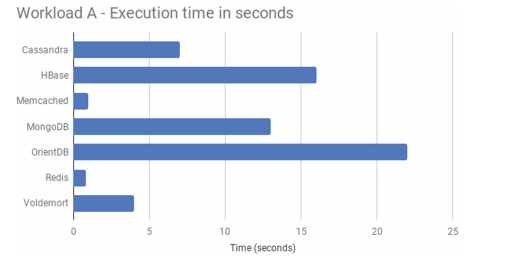
\includegraphics[width=0.9\linewidth]{figures/images/performance_a.png}
	\caption[6.000.000 rekord, 50\% olvasás, 50\% írás esetén]{\textit{6.000.000 rekord, 50\% olvasás, 50\% írás esetén}\footnotemark}
	\label{fig:performance_a}
\end{figure}

\footnotetext{https://www.researchgate.net/figure/Workload-A\_fig1\_332028074}

\begin{figure}[H]
	\centering
	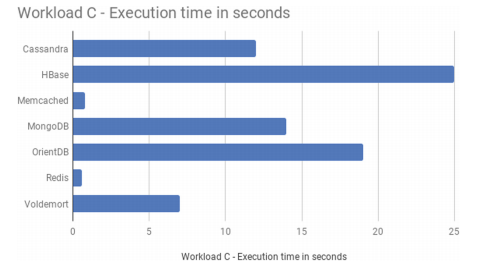
\includegraphics[width=0.9\linewidth]{figures/images/performance_b.png}
	\caption[6.000.000 rekord és 5.000 véletlenszerű olvasás esetén]{\textit{6.000.000 rekord és 5.000 véletlenszerű olvasás esetén}\footnotemark}
	\label{fig:performance_b}
\end{figure}

\footnotetext{https://www.researchgate.net/figure/Workload-C\_fig2\_332028074}

\begin{figure}[H]
	\centering
	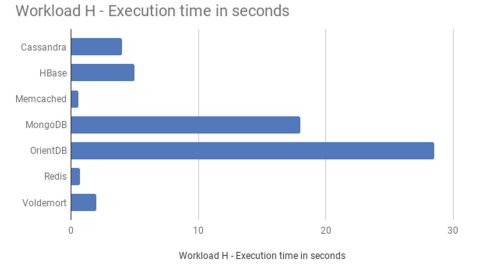
\includegraphics[width=0.9\linewidth]{figures/images/performance_c.png}
	\caption[6.000.000 rekord 5.000 véletlenszerű frissítés esetén]{\textit{6.000.000 rekord 5.000 véletlenszerű frissítés esetén}\footnotemark}
	\label{fig:performance_c}
\end{figure}

\footnotetext{https://www.researchgate.net/figure/Workload-H\_fig3\_332028074}
